\documentclass[t,xcolor={usenames,dvipsnames}]{beamer}

\mode<presentation>
{
\usetheme{Frankfurt}
%\setbeamercovered{transparent}
%\setbeamercolor{background canvas}{bg=white}
}

% Delete these, if you do not want the table of contents to pop up at
% the beginning of each (sub)section:
%\AtBeginSubsection[]
%{
%  \begin{frame}<beamer>{Outline}
%    \tableofcontents[currentsection,currentsubsection]
%  \end{frame}
%}
%\AtBeginSection[]
%{
%  \begin{frame}<beamer>{Outline}
%    \tableofcontents[currentsection]
%  \end{frame}
%}

\usepackage[english]{babel}
\usepackage[latin1]{inputenc}
\usepackage{times}
\usepackage[T1]{fontenc}
\usepackage{verbatim}
\usepackage{url}
\usepackage{amsmath,amssymb}
\usepackage{comment}
\usepackage{ifthen}

% Author-date citations
\usepackage[authoryear,round]{natbib}
\let\cite=\citep  % default \cite such as {\LaTeX} authors are used to

% Where \includegraphics should look for figures
\graphicspath{{./figs/}}
\usepackage{epstopdf}
\DeclareGraphicsExtensions{.eps,.png,.jpg,.pdf}

% Code
\usepackage{listings}
\lstloadlanguages{XML}
\lstset{language=XML}
\lstnewenvironment{blksedml}
    {\lstset{language=XML,basicstyle=\footnotesize}}
    {}
\newcommand{\sedml}[1]{\lstinline[basicstyle=\color{blue}]!#1!}

% Last package (safest!)
\usepackage{hyperref}

% Shortcuts
\newcommand{\myhref}[2]{\href{#1}{\textcolor{Blue}{#2}}}
\newcommand{\subitem}[1]{\begin{itemize}[<.->]\item #1 \end{itemize}}
\newcommand{\ghead}[1]{{\tiny #1\\}}
\newcommand{\doi}[2][]{\myhref{http://dx.doi.org/#2}{\ifthenelse{\equal{#1}{}}{doi:#2}{#1}}}
\newcommand{\csym}[1]{\textcolor{Blue}{\texttt{#1}}}

%%%%%%%%%%%%%%%%%%%%%%%%%%%%%%%%%%%%%%%%%%%%%%%%%%%%%%%%%%%%%%%%%%%%%%
\title{Possibilities for SED-ML}
\author[Jonathan Cooper]{Jonathan Cooper \and Gary Mirams \and James Osborne}
\institute[University of Oxford]
{Computational Biology Group\\
 Department of Computer Science\\
 University of Oxford}
\date{August 15, 2012}

\begin{document}

\begin{comment}
\begin{abstract}
We have been working on defining and using virtual experiments within a variety of contexts, including cardiac electrophysiology, multi-cellular tissue dynamics, immunology, and synthetic biology.  In doing so we have found that extensions are required if SED-ML is to address our needs.  This talk will introduce some of our use cases, highlight our functional curation framework (\url{https://chaste.cs.ox.ac.uk/cgi-bin/trac.cgi/wiki/FunctionalCuration}) for running experiments on a range of models, and outline our proposals for SED-ML.
\end{abstract}
\end{comment}

\begin{frame}
\titlepage
\end{frame}

%%%%%%%%%%%%%%%%%%%%%%%%%%%%%%%%%%%%%%%%%%%%%%%%%%%%%%%%%%%%%%%%%%%%%%

\begin{frame}{Outline}
\setcounter{tocdepth}{1}
\tableofcontents
\end{frame}


%%%%%%%%%%%%%%%%%%%%%%%%%%%%%%%%%%%%%%%%%%%%%%%%%%%%%%%%%%%%%%%%%%%%%%
\section[Introduction]{Introduction}
\subsection*{Main}
%%%%%%%%%%%%%%%%%%%%%%%%%%%%%%%%%%%%%%%%%%%%%%%%%%%%%%%%%%%%%%%%%%%%%%

\begin{frame}{What problem are we trying to solve?}
\begin{itemize}[<+->]
\item How can the whole modelling process be improved?
\item How can models be reused and composed reliably?
\item Especially as models increase in size and complexity
% Introduce cardiac application.  Make point that even cardiac cell model composed of many units at multiple levels: cell, ion channel, protein subunit.  Reaction networks also build complexity from small repeated concepts.
\end{itemize}
\begin{itemize}[<+->]
\item We want \ldots
  \begin{itemize}
  \item<.-> A single model description that can be used/analysed in multiple ways
  \item Separation of model structure (i.e.\ the equations describing biological function) and experimental scenario
  \item A uniform approach to model fitting, simulation, comparison and validation
  \end{itemize}
\end{itemize}
\end{frame}


\begin{frame}{Models, experiments and protocols}
\begin{itemize}
\item A \alert{model} is a purposeful simplification of reality
\item An \alert{experiment} is the process of stimulating a system to elicit observable responses
\item A \alert{protocol} is a detailed specification for carrying out an experiment
  \subitem{Environmental conditions / parameters, interventions, recordings, filtering \& post-processing, numerical algorithms, etc.}
\end{itemize}
\end{frame}


%%%%%%%%%%%%%%%%%%%%%%%%%%%%%%%%%%%%%%%%%%%%%%%%%%%%%%%%%%%%%%%%%%%%%%
\section[Use cases]{Use cases}
\subsection*{Main}
%%%%%%%%%%%%%%%%%%%%%%%%%%%%%%%%%%%%%%%%%%%%%%%%%%%%%%%%%%%%%%%%%%%%%%

\begin{frame}{Use cases}
\begin{itemize}
\item Functional curation of cardiac cell models
\item Parameter sweeping models of multi-cellular tissue dynamics
\item Experiments in immunology and synthetic biology
 % Won't talk about this in detail, just mention, along with text syntax
\end{itemize}
\end{frame}


\begin{frame}{Functional curation of cardiac models}
This use case was also described last year.
Focus on a protocol that demonstrates some features we've added since
--- finding a ``steady state'' for a given pacing rate.
\end{frame}


\begin{frame}{Intestinal crypt --- cell-based Chaste}
Show 3d node-based crypt movie, and talk around it.
Refer back to Ozzy's talk.
Look at distribution of cell division events in space, cell ages at division.
Look at effects of parameter variation on whether mutant invades or is swept out.
Look at how these results vary across models.
\end{frame}


\begin{frame}{Our framework}
% This may be better at end of intro?
\begin{center}
\vspace{-.5cm}\hspace*{-.75cm}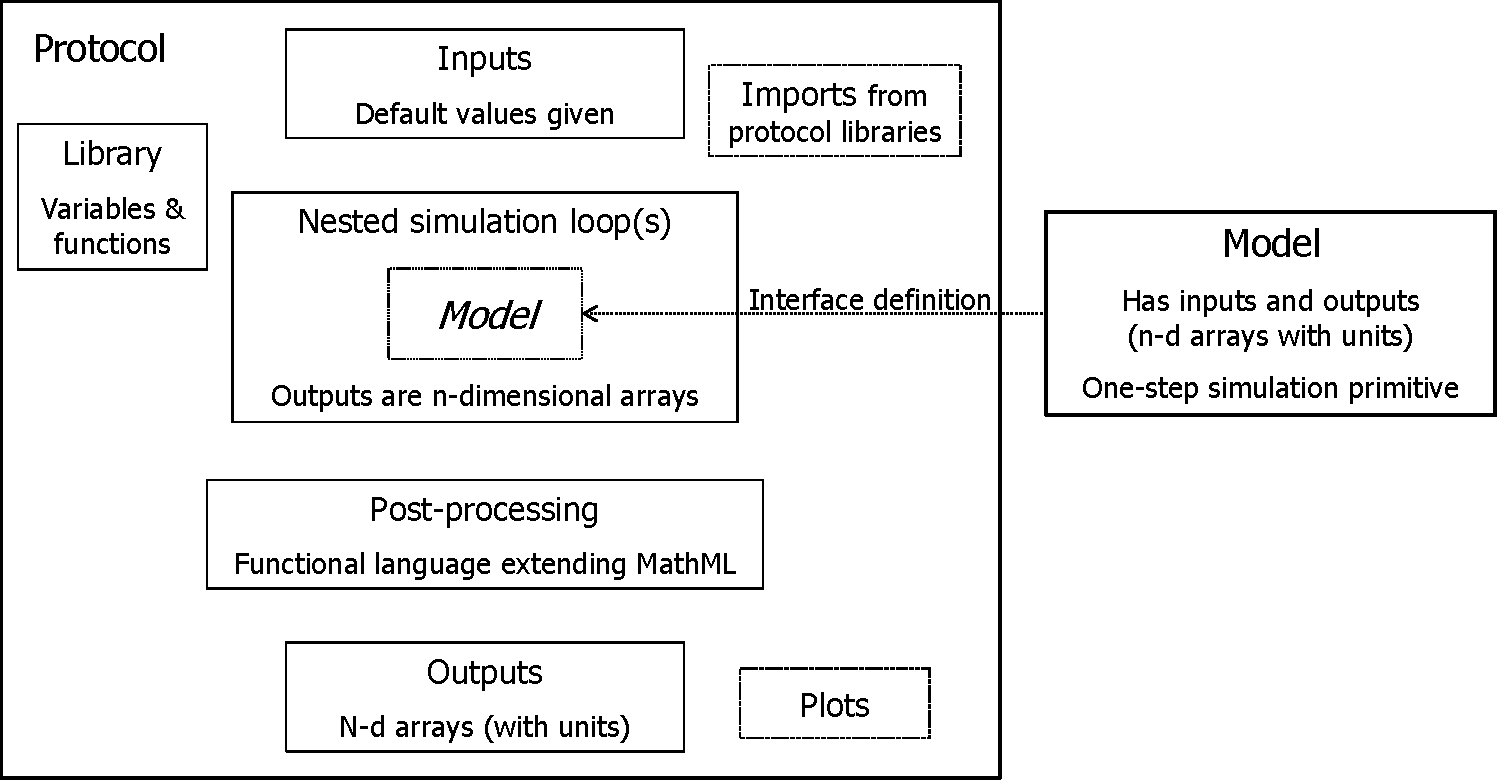
\includegraphics[width=1.15\textwidth]{proto_diag}
\end{center}
\end{frame}

%%%%%%%%%%%%%%%%%%%%%%%%%%%%%%%%%%%%%%%%%%%%%%%%%%%%%%%%%%%%%%%%%%%%%%
\section{Proposals for SED-ML}
\subsection*{Main}
%%%%%%%%%%%%%%%%%%%%%%%%%%%%%%%%%%%%%%%%%%%%%%%%%%%%%%%%%%%%%%%%%%%%%%

\begin{frame}{Some proposals for SED-ML}
\begin{itemize}
\item \hyperlink{prop:anymodel}{Applying a protocol to any model}
  \subitem{\hyperlink{prop:onto}{Using ontological annotations}}
\item \hyperlink{prop:tasks}{New task hierarchy}
  \subitem{Split up \sedml{repeatedTask}}
\item \hyperlink{prop:varref}{Extending variable references}
  \subitem{Chaining post-processing}
\item \hyperlink{prop:nd}{Handling n-dimensional data}
\end{itemize}
\end{frame}

%%%%%%%%%%%%%%%%%%%%%%%%%%%%%%%%%%%%%%%%%%%%%%%%%%%%%%%%%%%%%%%%%%%%%%

\begin{frame}<1>[label=prop:anymodel]{Applying a protocol to any model}
\alert{Problem}:
 In order to compare models under a given protocol, we require that
 the protocol does not hardcode the model to use.

\alert{Proposal}:
 Allow the \sedml{source} attribute on \sedml{model} to hold a special
 SED-ML URN, \sedml{urn:sedml:anymodel} say, that signals to
 processing software that the specific model must be supplied by some
 external mechanism.
\end{frame}

%%%%%%%%%%%%%%%%%%%%%%%%%%%%%%%%%%%%%%%%%%%%%%%%%%%%%%%%%%%%%%%%%%%%%%

\begin{frame}<1>[label=prop:onto]{Extending variable references (1)}
\alert{Problem}:
 Different models may use different names for the same concept.  How
 can a single protocol be applied to both?

 \alert{Ontological annotation} can provide a consistent nomenclature.

 Model and protocol need to agree on ontology to use.

\alert{Proposal}:
 Allow the \sedml{variable} element to use an ontology term instead of
 an XPath expression.

 Either in the \sedml{target} attribute itself, or a new
 \sedml{annotatedTarget} attribute.
\end{frame}

%%%%%%%%%%%%%%%%%%%%%%%%%%%%%%%%%%%%%%%%%%%%%%%%%%%%%%%%%%%%%%%%%%%%%%

\begin{frame}<1>[label=prop:tasks]{New task hierarchy}
\alert{Problem}:
 Frank's proposed \sedml{repeatedTask} conflates multiple concepts:
\begin{itemize}
\item Associating a model with a simulation
\item Repeating a task (potentially with changes)
\item Grouping tasks to be run together (in sequence or parallelisable)
\end{itemize}

\alert{Proposal}:
 Separate them into 3 task classes, inheriting from a common abstract
 class.

TODO: Simple UML-like diagram
\end{frame}


\begin{frame}[fragile=singleslide]
\frametitle{Examples (1)}
\begin{blksedml}
<!-- Test when order matters -->
<combinedTask id="seq" scheduling="sequential">
    <listOfSubTasks>
        <subTask task="task1" resetModel="false"/>
        <subTask task="task2" resetModel="false"/>
    </listOfSubTasks>
</combinedTask>

<!-- Test when order does not matter -->
<combinedTask id="para" scheduling="parallel">
    <listOfSubTasks>
        <subTask task="task1" resetModel="true"/>
        <subTask task="task2" resetModel="true"/>
    </listOfSubTasks>
</combinedTask>
\end{blksedml}
\end{frame}
        
\begin{frame}[fragile=singleslide]
\frametitle{Examples (2)}
\begin{blksedml}
<!-- Test nesting a combined task -->
<nestedTask id="nested" resetModel="false"
            range="loop_counter">
    <listOfRanges>
        <vectorRange id="loop_counter">
            <value>0</value>
            <value>1</value>
            <value>2</value>
        </vectorRange>
    </listOfRanges>
    <subTask task="seq"/>
</nestedTask>
        
<!-- Test combined inside combined -->
<combinedTask id="c_in_c" scheduling="sequential">
    <listOfSubTasks>
        <subTask task="seq" resetModel="false"/>
    </listOfSubTasks>
</combinedTask>
\end{blksedml}
\end{frame}


\begin{frame}[fragile=singleslide]
\frametitle{Getting the results out}
\alert{Problem}:
 Repeated and combined tasks lead to more complex results data
 structures than the 2d arrays in SED-ML L1V1.

\begin{itemize}
\item Repeated tasks yield n-dimensional arrays --- see next section
\item Combined tasks yield ``sub-results''
\end{itemize}

\alert{Proposal}:
 Enhance the \sedml{taskReference} attribute on \sedml{variable} to be
 able to indicate sub-tasks,
 e.g.\ \sedml{taskReference='task:subtask'}.

Continuing the earlier example:
\begin{blksedml}
<variable id="V1_V" taskReference="seq:task1"
          target="..."/>
\end{blksedml}
\end{frame}

%%%%%%%%%%%%%%%%%%%%%%%%%%%%%%%%%%%%%%%%%%%%%%%%%%%%%%%%%%%%%%%%%%%%%%

\begin{frame}<1>[label=prop:varref]{Extending variable references (2)}
\alert{Problem}:
 Sometimes we want to refer to variables defined in the
 \emph{protocol}, not the model.

\begin{itemize}
\item
 Data generators cannot currently take the outputs of other data
 generators as inputs.
\item
 Changes in nested tasks need to refer to range values.
\end{itemize}

\alert{Proposal}:
 Most SED-ML elements already have an \sedml{id} attribute.

 Allow the \sedml{variable} element to reference these, either with
 \sedml{target='\#id'}, or a new attribute \sedml{idref}.
 % FB used target="#current" in the nested proposal v3
\end{frame}


\begin{frame}{Extending variable references (3)}
% This needs to be after the new task hierarchy
\alert{Problem}:
 We might want to vary algorithm parameters over a repeated task.

\alert{Proposal}:
 If \sedml{algorithmParameter} gains an (optional) \sedml{id}, the
 referencing scheme proposed earlier suffices.

Example: a timecourse simulation implemented using a repeated task.
(TODO)
\end{frame}

%%%%%%%%%%%%%%%%%%%%%%%%%%%%%%%%%%%%%%%%%%%%%%%%%%%%%%%%%%%%%%%%%%%%%%

\begin{frame}<1>[label=prop:nd]{Handling n-dimensional data}
TODO
\end{frame}


%%%%%%%%%%%%%%%%%%%%%%%%%%%%%%%%%%%%%%%%%%%%%%%%%%%%%%%%%%%%%%%%%%%%%%
\section{Ideas for future proposals}
\subsection*{Main}
%%%%%%%%%%%%%%%%%%%%%%%%%%%%%%%%%%%%%%%%%%%%%%%%%%%%%%%%%%%%%%%%%%%%%%

\begin{frame}{Looking further ahead}
\begin{itemize}[<+->]
\item Units conversions
  \subitem{Requires a units standard across modelling languages}
\item Protocol libraries
\item Dealing with irregular data
  \subitem{e.g.\ arising from cell birth and death}
\end{itemize}
\end{frame}


%%%%%%%%%%%%%%%%%%%%%%%%%%%%%%%%%%%%%%%%%%%%%%%%%%%%%%%%%%%%%%%%%%%%%%
\section{Conclusions}
\subsection*{Main}
%%%%%%%%%%%%%%%%%%%%%%%%%%%%%%%%%%%%%%%%%%%%%%%%%%%%%%%%%%%%%%%%%%%%%%

\begin{frame}{Current threads of work}
TODO: some wrapping up text
\begin{itemize}
\item Improving implementation
  \subitem{Including a simple graphical interface for running experiments and querying results}
\item Developing new protocol concepts as needed by applications
\item Textual syntax for protocol language
\item Developing SED-ML extensions
\item Encoding protocols for cardiac electrophysiology, cell-based Chaste, immunology, synthetic biology, \ldots
\end{itemize}
\end{frame}


\begin{frame}{Acknowledgments}
Chaste team\\
Alan Garny, Steven Niederer, Mark Slaymaker

Reference publication: \doi[Prog Biophys Mol Biol 107:11-20, 2011]{10.1016/j.pbiomolbio.2011.06.003}\\
Web site: \url{https://chaste.cs.ox.ac.uk/cgi-bin/trac.cgi/wiki/FunctionalCuration}

\begin{center}

\includegraphics[scale=.9]{chaste-266x60}\\ \vspace{.4cm}

\includegraphics[height=.42cm]{EPSRC1RGBLO} \hspace{.05cm}

\includegraphics[height=.42cm]{logo_msr} \hspace{.05cm}

\includegraphics[height=.42cm]{logo2020science}\\ \vspace{.2cm}

\includegraphics[height=1.1cm]{FP7-gen-RGB}
\end{center}
\end{frame}

\end{document}
